\documentclass{report}
\usepackage{subfiles}
\usepackage[latin1]{inputenc}
\usepackage[english]{babel}
\usepackage[T1]{fontenc}
\usepackage{amsmath,amssymb}
\usepackage{fancyhdr}
\usepackage{hyperref}
\usepackage{graphicx}
\usepackage{tabularx}
\usepackage{float}
\usepackage{color}
\usepackage{enumitem}
\usepackage{nameref}
\usepackage{caption}
\usepackage{parskip}
\usepackage{placeins}
\usepackage{pdflscape}
\usepackage{geometry}
\usepackage{listings}
\definecolor{bluekeywords}{rgb}{0.13,0.13,1}
\definecolor{greencomments}{rgb}{0,0.5,0}
\definecolor{redstrings}{rgb}{0.9,0,0}
\lstset{language=[Sharp]C,
  showspaces=false,
  showtabs=false,
  breaklines=true,
  showstringspaces=false,
  breakatwhitespace=true,
  escapeinside={(*@}{@*)},
  commentstyle=\color{greencomments},
  keywordstyle=\color{bluekeywords},
  stringstyle=\color{redstrings},
  basicstyle=\ttfamily
}


\setcounter{secnumdepth}{3}
\setcounter{tocdepth}{2}

\makeatletter



\def\twodigits#1{\expandafter\two@digits\csname c@#1\endcsname}

\AddEnumerateCounter\twodigits\two@digits{01}

\makeatother


\fancyfoot[OC]{\textit{\thepage}}

\title{Sample Title}
\date{\today}
\author{Asbj\o rn Fjelbro Steffensen (afjs@itu.dk)\\ Thomas Stoy Dragsb\ae k (thst@itu.dk)\\ Nicki Hjorth J\o rgensen (nhjo@itu.dk)\\ Jacob Benjamin Cholewa (jbec@itu.dk)\\ Jakob Merrild (jmer@itu.dk)\\ Mathias Kindsholm Pedersen (mkin@itu.dk)}

\begin{document}

\begin{titlepage}
\begin{center}

\vspace{2cm}

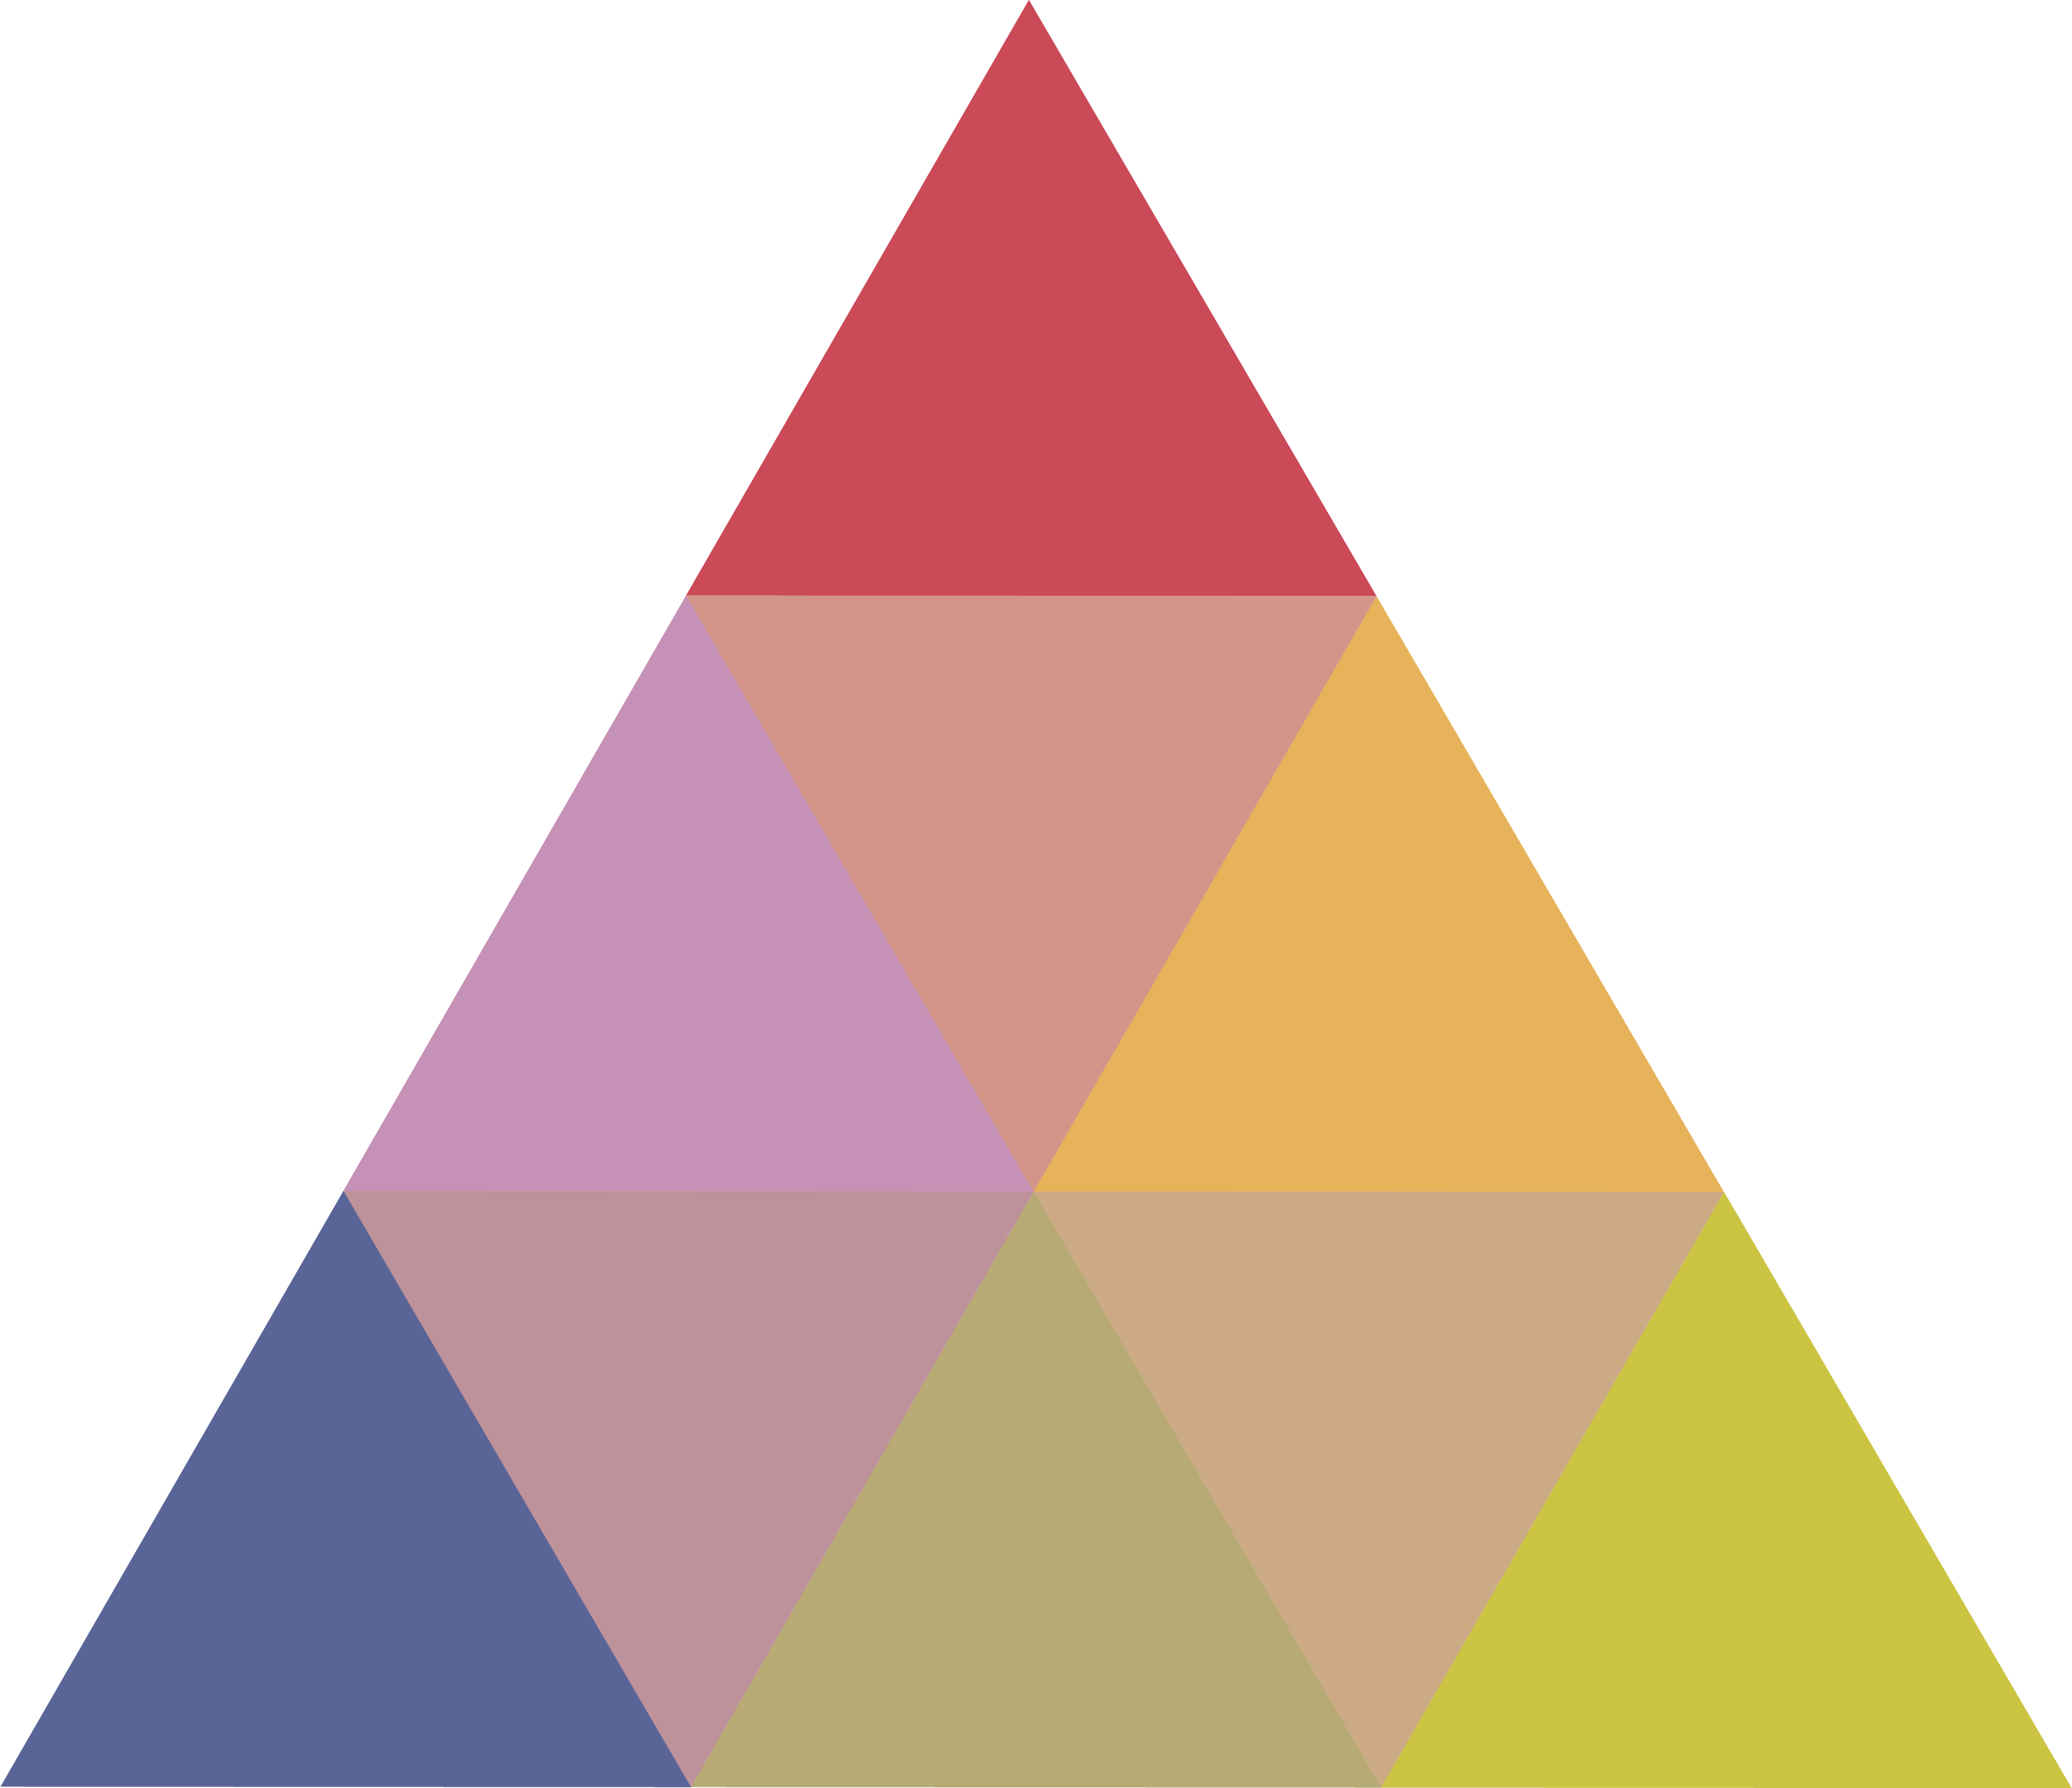
\includegraphics[scale=0.5]{./img/logo.png}

\rule{\linewidth}{0.6mm}

\textsc{\LARGE ShareIT and ArtShare} \\
\textsc{Software Development in Large Teams with International Collaboration(BNDN)}
\vspace{0.2cm}
\rule{\linewidth}{0.4mm}

Asbj\o rn Fjelbro Steffensen (afjs@itu.dk)\\ Thomas Stoy Dragsb\ae k (thst@itu.dk)\\ Nicki Hjorth J\o rgensen (nhjo@itu.dk)\\ Jacob Benjamin Cholewa (jbec@itu.dk)\\ Jakob Merrild (jmer@itu.dk)\\ Mathias Kindsholm Pedersen (mkin@itu.dk)

\vfill

\large \today
\end{center}


\end{titlepage}
\newpage
\tableofcontents

\chapter{Glossary}
\subfile{tex/glossary.tex}

\chapter{Introduction}
\subfile{tex/introduction.tex}

\newpage
\subfile{tex/businessCase.tex}

\chapter{Proposed System}

\section{Overview}

!!! SHOULD BE REVISED !!!

The proposed system is to handle different types of media files (e.g. books, video, sound or images). It must be extendable, such that any given client can upload and search for the most common types of media.

The systems functionality is aimed for anyone that uses their computer as a media center. This is, users that has a collection of books, video-, sound- or imagefiles on their computer or mobile devices.

\section{Scope of the system}
\subfile{tex/scope.tex}

\section{Requirement specification}
\subsection{Section overview}
This section will describe elicitation of requirements for both AreShare (Our client implementation) and our shareIT back-end API. As it is a part of the project requirements, the shareIT API will be build so that other client implementations can be build on top of the existing API.

In this section only scenarios, use cases, and function requirements to our part of the platform will be discussed, but shareIT requirements will be influenced by external requirements from a third-party 

The following describes scenarios of what end-users will be able to do on the platform followed by use cases and functional requirements derived from these scenarios.


% SCENARIOS SECTION %
\subsection{Scenarios}
\documentclass[../report.tex]{subfiles}



\begin{document}


\section{Actors}
\begin{itemize}
\item \textbf{Admin} \\
The Admin has access to all content and is able to delete content if necessary. 
\item \textbf{Anonymous user}\\ 
The Anonymous User is an anonymous client of the system. This actor is not able to use all functionality of the system. Only browsing the content is allowed
\item \textbf{User} \\
The User is an registered and identified client of the system. The user has created an account which he is logged into. This user is allowed to do more than the Anonymous User. This includes uploading, purchasing and rating content and managing account information and content uploaded by the User.
\end{itemize}

\section{User Stories}
\begin{itemize}
\item UploadContent \\
John is an anonymous user of RentIt. He wants to upload "Sinful Summer", a movie he has made, so he can make some money from it. In order to be able to do so he must register a user with the system. He registers a user called John33. John33 finds the movie file he wants to upload and enters information about it into the system. He then uploads the movie.
\item PurchaseContent \\
Robert is an anonymous user of RentIt. He wants to purchase "War and Peace" as an ebook. He uses the search function to find the ebook he is looking for. In order to be able to purchase the ebook he must log in. Robert already has a user called Robbie93 so he logs in as Robbie93. Robbie93 purchases the ebook and downloads it.
\item RateContent \\
Daniel54 is a registered RentIt user. He has previously purchased and listened to the Pink Floyd song "Money". He thought it was a great song and he wants to let the other users of RentIt know about this. He finds "Money" using the search function. He then uses the rating system to give it a high rating.
\item ManageUploadedContent \\
Bob1970, a registered user of RentIt, notices that he made a spelling error in the title of the music track he just uploaded. He changes the title from "Parise the Lord" to "Praise the Lord" and saves the changes.
\item ManageAccount \\
Kelly89 is a registered user of RentIt. When Kelly89 registered with RentIt, she did not fill the description of her account. She now wants to add a description so that other users can see what to expect from her account. She updates the description and saves the changes.
\item DeleteContent \\
Anna, an admin of RentIt, browses through the content and finds a suspicious movie called "Sinful Summer". Anna watches the movie and finds out that the movie violates the law. Anna deletes the movie.
\end{itemize}

\section{Use Cases}
Anonymous: Search, CreateAccount \\
User: Search, Login, Logout, Upload, Purchase, Rate, EditUserAccountInfo, EditContentInfo, Download \\
Admin: DeleteContent, Search, Login, Logout, EditUserAccountInfo, EditContentInfo, Download

\end{document}

% USE CASE SECTION %
\newpage
\subsection{Use Cases}
\FloatBarrier
%\documentclass[../report.tex]{subfiles}
%\begin{document}

%\addtolength{\topmargin}{-1in}

%Anonymous: Search, CreateAccount, Login \\
%User: Search, Logout, Upload, Purchase, Rate, EditUserAccountInfo, EditContentInfo, Download \\
%Admin: DeleteContent, Search, Logout, EditUserAccountInfo, EditContentInfo, Download \\
% Search, CreateAccount, Login, Logout, Upload, Purchase, Rate, EditUserAccountInfo, EditContentInfo, Download, DeleteContent

\captionsetup[table]{labelformat=empty}
\captionsetup[table]{font=large}
\captionsetup[table]{textfont=bf}

\noindent
\begin{table}[h!]
\caption{UC-01}
\label{UC-01}
\begin{tabular}{ l  p{8cm} }  
\hline
\\
Use case name:  & RateMedia   \\   \hline    
\\            
Participating actors:  & \texttt{\texttt{User}} \\   \hline   
\\             
Flow of events: & \begin{enumerate}
\item{The \texttt{User} finds the \textit{Media} to be rated and navigates to its \textit{Details Page}}
\item{The \texttt{User} chooses to rate this \textit{Media}}
\item{The \texttt{User} is presented with a rating form where he selects a rating to give the \textit{Media}}
\item{The \textit{System} saves the rating of the \textit{Media} and notifies the \texttt{User} of this}
\end{enumerate}
\\ \hline
\\
Rules: & Each \texttt{User} can only rate the same \textit{Media} once
\\   \hline 
\\
Entry condition: & \texttt{User} must be logged in \\ \hline
\\
Exit condition: & The \textit{Media} has been rated \\ \hline
\\
Quality requirements: & The \textit{System} must reflect the changes to the rating and notify the \texttt{User} within 5 seconds of the
\texttt{User} submitting the rating\\ \hline  
\end{tabular}
\end{table}

\noindent
\begin{table}[h!]
\caption{UC-02}
\label{UC-02}
\begin{tabular}{ l  p{8cm} } 
\hline 
\\
Use case name:  & EditUserAccountInfo   \\   \hline    
\\            
Participating actors:  & \texttt{User, \texttt{Admin}} \\   \hline   
\\      
Flow of events: & \begin{enumerate}
\item{The \texttt{Actor} navigates to the \textit{Account Page} of the \textit{Account} which info is to be edited}
\item{The \texttt{Actor} initiates the editing of this \textit{Account}}
\item{The \texttt{Actor} is presented with a form containing \textit{Account Information}}
\item{The \texttt{Actor} edits whatever information he wants in the form}
\item{The \texttt{Actor} either chooses to discard the changes or to save them}
\item{The \texttt{Actor} is redirected to the \textit{Account Page}}
\end{enumerate}
\\
Alternatives: & \begin{itemize}
\item[\textbf{5a:}]{\textbf{The \texttt{Actor} saves the changes}}
\item[]  5a1. The changes are saved by the \textit{System}
\item[\textbf{5b:}]\textbf{The \texttt{Actor} discards the changes}
\item[]  5b1. The changes are not saved by the \textit{System}
\end{itemize}
\\ \hline
\\
Rules: & \texttt{Users} can only edit their own \textit{Account} information whereas \texttt{Admins} can edit the information of any  \textit{Account}
\\   \hline 
\\
Entry condition: & The \texttt{Actor} must be logged in \\ \hline
\\
Exit condition: & The \textit{Account}'s info has been changed and the \textit{System} has been updated to reflect these changes OR
nothing has changed if the \texttt{Actor} discarded the changes\\ \hline
\\
Quality requirements: & The \textit{System} must reflect the changes to the \textit{Account} and notify the \texttt{User} within 5 seconds of the \texttt{User} submitting the changes \\ \hline  
\end{tabular}
\end{table}

\noindent
\begin{table}[h!]
\caption{UC-03}
\label{UC-03}
\begin{tabular}{ l  p{8cm} }  
\hline
\\
Use case name:  & EditMediaInfo   \\   \hline    
\\            
Participating actors:  & \texttt{\texttt{User}, \texttt{Admin}} \\   \hline   
\\             
Flow of events: & \begin{enumerate}
\item{The \texttt{Actor} navigates to the \textit{Details Page} of the \textit{Media} which info is to be edited}
\item{The \texttt{Actor} initiates the editing of this \textit{Media}}
\item{The \texttt{Actor} is presented with a form containing \textit{Media Item Information}}
\item{The \texttt{Actor} edits whatever information he wants in the form}
\item{The \texttt{Actor} either chooses to discard the changes or to save them}
\item{The \texttt{Actor} is redirected to the \textit{Details Page} of the \textit{Media} that has been edited}
\end{enumerate}
\\
Alternatives: & \begin{itemize}
\item[\textbf{5a:}]{\textbf{The \texttt{Actor} saves the changes}}
\item[]  5a1. The changes are saved by the \textit{System}
\item[\textbf{5b:}]{\textbf{The \texttt{Actor} discards the changes}}
\item[]  5b1. The changes are not saved by the \textit{System}
\end{itemize}
\\ \hline
\\
Rules: & \texttt{Users} can only edit the information of the \textit{Media} they have uploaded whereas \texttt{Admins} can edit the information of all \textit{Media}
\\   \hline 
\\
Entry condition: & The \texttt{Actor} must be logged in \\ \hline
\\
Exit condition: & The \textit{Media}'s info has been changed and the \textit{System} has been updated to reflect these changes OR
nothing has changed if the \texttt{Actor} discarded the changes \\ \hline
\\
Quality requirements: & The \textit{System} must reflect the changes to the \textit{Account} and notify the \texttt{User} within 5 seconds of the \texttt{User} submitting the changes \\ \hline  
\end{tabular}
\end{table}

\noindent
\begin{table}[h!]
\caption{UC-04}
\label{UC-04}
\begin{tabular}{ l  p{8cm} }   
\hline
\\
Use case name:  & DownloadMedia   \\   \hline    
\\            
Participating actors:  & \texttt{\texttt{User}, \texttt{Admin}} \\   \hline   
\\             
Flow of events: & \begin{enumerate}
\item{The \texttt{Actor} navigates to the \textit{Details Page} for the \textit{Media} which is to be downloaded}
\item{The \texttt{Actor} initiates the download of the \textit{Media}}
\item{The \textit{System} transfers the file containing the \textit{Media} to the \texttt{Actor}'s local hard drive}
\end{enumerate}
\\ \hline
\\
Rules: & \texttt{Users} can only download \textit{Media} that they have gained access to by purchasing it whereas \texttt{Admins} can download all \textit{Media}
\\   \hline 
\\
Entry condition: & The \texttt{Actor} must be logged in \\ \hline
\\
Exit condition: & The \texttt{Actor} has received the \textit{Media} \\ \hline
\\
Quality requirements: & N/A  \\ \hline
\end{tabular}
\end{table}

\noindent
\begin{table}[h!]
\caption{UC-05}
\label{UC-05}
\begin{tabular}{ l  p{8cm} }
\hline                        
\\
Use case name:  & DeleteMedia   \\   \hline    
\\            
Participating actors:  & \texttt{Admin} \\   \hline   
\\             
Flow of events: & \begin{enumerate}
\item{The \texttt{Admin} navigates to the \textit{Details Page} of the \textit{Media} which is to be deleted}
\item{The \texttt{Admin} is asked to confirm the deletion of the \textit{Media}}
\item{The \texttt{Admin} chooses whether or not to delete the \textit{Media}}
\end{enumerate}
\\
Alternatives: & \begin{itemize}
\item[\textbf{3a:}]{\textbf{The \texttt{Admin} confirms the deletion of the \textit{Media}}}
\item[]  3a1. The file is deleted and the \textit{System} is updated to reflect that the \textit{Media} is no longer available
\item[\textbf{3b:}]{\textbf{The \texttt{Admin} cancels the deletion of the \textit{Media}}}
\item[]  3b1. No changes are saved by the \textit{System} and the \texttt{Admin} is redirected to the \textit{Details Page} of the \textit{Media} which was to be deleted
\end{itemize}
\\ \hline
\\
Rules: & N/A
\\   \hline 
\\
Entry condition: & \texttt{Admin} must be logged in \\ \hline
\\
Exit condition: & The file containing the \textit{Media} has been deleted and the \textit{System} has been updated to reflect these changes \\ \hline
\\
Quality requirements: & N/A \\ \hline  
\end{tabular}
\end{table}

\noindent
\begin{table}[h!]
\caption{UC-06}
\label{UC-06}
\begin{tabular}{ l p{8cm} } 
\hline  
\\                   
Use case name:  & Search   \\   \hline \\                
Participating actors:  & \texttt{Anonymous user, User, Admin} \\   \hline \\
Flow of events: & \begin{enumerate}
\item{The \texttt{Actor} enters a search keyword and initiates the search}
\item{The \texttt{Actor} is presented with the search results}
\item{The \texttt{Actor} picks the desired search result or tries again with another search keyword}
\end{enumerate} \\
Alternatives: & \begin{itemize}
\item[\textbf{3a:}] \textbf{The \texttt{Actor} picks the desired search result}
\item[]  3a1. The \textit{Details page} of the desired search result is shown by \textit{The System}
\item[\textbf{3b:}] \textbf{The \texttt{Actor} tries again with another search keyword}
\item[]  3b1. The \texttt{Actor} is back at step 2.
\end{itemize} \\ 
\hline \\
Rules: & N/A \\ \hline \\
Entry condition: & N/A \\ \hline \\
Exit condition: & The \texttt{Actor} has found the result he was looking for or he is certain that the search keyword did not help him find what he was looking for \\ \hline \\
Quality requirements: & The search results (if any) must be presented within 5 seconds from initiating search \\ \hline           
\end{tabular}
\end{table}

\noindent
\begin{table}[h!]
\caption{UC-07}
\label{UC-07}
\begin{tabular}{ l p{8cm} } 
\hline       
\\                
Use case name:  & CreateAccount   \\   \hline  \\              
Participating actors:  & \texttt{Anonymous user} \\   \hline \\
Flow of events: & \begin{enumerate}
\item{The \texttt{Anonymous user} initiates the creation of an \textit{Account}}
\item{The \texttt{Anonymous user} is presented with a form to fill}
\item{The \texttt{Anonymous user} fills out the form by entering Username, Password and any of the optional \textit{Account Information} before submitting} %update when account information is known 
\item{The \texttt{Anonymous user} is notified that the \textit{Account} is created}
\end{enumerate}
\\   \hline \\
Rules: & The \textit{Account} must have a unique user name and email \\ \hline \\
Entry condition: & The \texttt{Anonymous user} has no \textit{Account} \\ \hline \\
Exit condition: & The \texttt{Anonymous user} has created an \textit{Account} \\ \hline \\
Quality requirements: & The \textit{Account} must be created within 5 seconds from submitting \\  \hline      
\end{tabular} \\
\end{table}

\noindent
\begin{table}[h!]
\caption{UC-08}
\label{UC-08}
\begin{tabular}{ l p{8cm} }
\hline             
\\    
Use case name:  & Login   \\   \hline \\            
Participating actors:  & \texttt{Anonymous user, User} \\   \hline \\   
Flow of events: & \begin{enumerate}
\item{The \texttt{Anonymous user} initiates the login}
\item{The \texttt{Anonymous user} is presented with a login form}
\item{The \texttt{Anonymous user} enters his user name and password before submitting}
\end{enumerate} \\
Alternatives: & \begin{itemize}
\item[\textbf{3a:}] \textbf{The \texttt{Anonymous user} enters the correct user name and password}
\item[]  3a1. The \texttt{Anonymous user} is logged in and becomes a \texttt{User}
\item[\textbf{3b:}] \textbf{The \texttt{Anonymous user} enters the incorrect user name or password}
\item[]  3b1. The \texttt{Anonymous user} is notified that the user name or password was incorrect
\end{itemize} \\ 
\hline \\
Rules: & N/A \\ \hline \\
Entry condition: & The \texttt{Anonymous User} is not logged in \\ \hline \\
Exit condition: & The \texttt{Anonymous user} has been logged in to his \textit{Account} and is now a \texttt{User} or the \texttt{Anonymous user} is notified that the user name or password is incorrect \\ \hline \\
Quality requirements: & The \texttt{Anonymous user} must be logged in within 5 seconds from submitting provided that user name and password are correct \\ \hline \\            
\end{tabular} \\
\end{table}

\noindent
\begin{table}[h!]
\caption{UC-09}
\label{UC-09}
\begin{tabular}{ l p{8cm} }  
\hline           
\\       
Use case name:  & Logout   \\   \hline \\               
Participating actors:  & \texttt{User, Anonymous user} \\   \hline \\         
Flow of events: & \begin{enumerate}
\item{The \texttt{User} initiates the logout}
\item{The \texttt{User} is notified that he has logged out}
\item{The \texttt{User} is now an \texttt{Anonymous user}}
\end{enumerate}
\\   \hline \\
Rules: & N/A \\ \hline \\
Entry condition: & The \texttt{User} is logged in \\ \hline \\
Exit condition: & The \texttt{User} is no longer logged in and is therefore an \texttt{Anonymous user} \\ \hline \\
Quality requirements: & The \texttt{User} must be logged out within 5 seconds from initiating the logout \\ \hline             
\end{tabular} \\
\end{table}
\\ \\ \\

\noindent
\begin{table}[h!]
\caption{UC-10}
\label{UC-10}
\begin{tabular}{ l p{8cm} } 
\hline  
\\                   
Use case name:  & Upload   \\   \hline \\               
Participating actors:  & \texttt{User} \\   \hline \\         
Flow of events: & \begin{enumerate}
\item{The \texttt{User} initiates the upload}
\item{The \texttt{User} is presented with a form to fill}
\item{The \texttt{User} chooses the \textit{Media} he wishes to upload. He enters the Type which is a required field and any of the optional \textit{Media Item Information} of the \textit{Media} before submitting}
\end{enumerate} \\
Alternatives: & \begin{itemize}
\item[\textbf{3a:}] \textbf{The \textit{Media} is accepted}
\item[]  3a1. The \texttt{User} is notified that the \textit{Media} is being uploaded
\item[\textbf{3b:}] \textbf{The \textit{Media} is not accepted}
\item[]  3b1. The \texttt{User} is notified that the \textit{Media} is not accepted
\end{itemize}
\\   \hline \\
Rules: & N/A \\ \hline \\
Entry condition: & The \texttt{User} is logged in and he has the desired \textit{Media} locally on his system \\ \hline \\
Exit condition: & The \texttt{User} has uploaded the desired \textit{Media} \\ \hline \\
Quality requirements: & N/A \\ \hline \\
\end{tabular} \\
\end{table}

\noindent
\begin{table}[h!]
\caption{UC-11}
\label{UC-11}
\begin{tabular}{ l p{8cm} }   
\hline             
\\
Use case name:  & Purchase   \\   \hline \\                
Participating actors:  & \texttt{User} \\   \hline \\         
Flow of events: & \begin{enumerate}
\item{The \texttt{User} initiates the purchase of the selected \textit{Media}}
\item{The \texttt{User} is notified that the \textit{Media} has been bought}
\item{The \texttt{User} will now be able to download the \textit{Media}}
\end{enumerate}
\\
\hline \\
Rules: & N/A \\ \hline \\
Entry condition: & The \texttt{User} is logged in \\ \hline \\
Exit condition: & The \texttt{User} has bought the desired \textit{Media} or is notified that he does not have enough coins to buy the \textit{Media} \\ \hline \\
Quality requirements: & The \textit{Media} must be purchased within 5 seconds from initiating the purchase \\ \hline             
\end{tabular} \\
\end{table}

%\end{document}

% FUNCTION REQUIREMENTS

\FloatBarrier
\newpage \subsection{Functional Requirements - ArtShare}
\documentclass[../report.tex]{subfiles}



\begin{document}

\section{Functional Requirements}

\subsection {Search}

\begin{enumerate}[label=FR-\twodigits*]

	\item All \textbf{users} must be able to initiate a search by providing a keyword or key-phrase.
	\item The keyword or key-phrase must be matched with \textit{media} on title and artist/user.
	\item The \textbf{user} must be presented with all matches.
	\item Each match must include a link to a detailed page about the \textit{medium}.
	\item Matches must be grouped by media type. 
\end{enumerate}	
			
\subsection{Create account}

\begin{enumerate}[label=FR-\twodigits*, resume]
	\item An anonymous user must be able to create an account.
	\item To create an account the user must provide a desired username and password.
	\item Usernames must be unique with case insensitive matching. \label{FR-CA.3}
	\item A user must be given an alert if the desired username is unavailable.
	\item A username must consist of between 1 and 20 characters.
	\item A username must only consist of alphanumeric characters (a-zA-z0-9).
	\item A password must consist of between 1 and 50 characters. \label{FR-CA.7}
	\item If requirements \ref{FR-CA.3} - \ref{FR-CA.7} is not met a warning must be displayed to the user.
\end{enumerate}
	
\subsection {Login}
	
\begin{enumerate}[label=FR-\twodigits*, resume]
	\item A registered user must be able to login to the system providing a username and password pair.
	\item If the username and password pair is not matched an error message must be provided to the user. 
\end{enumerate}
		
\subsection {Manage account}

\begin{enumerate}[label=FR-\twodigits*, resume]
	\item A logged-in user must be able to edit all profile information on his own account excluding username.
	\item A administrator must be able to edit all profile information of all accounts excluding usernames.
	\item Changes to a users password must still comply with requirement \ref{FR-CA.7} \label{FR-MA.2}
	\item A warning must be displayed to the user if requirement \ref{FR-MA.2} is not met.	
\end{enumerate}
		
\subsection {Logout}
\begin{enumerate}[label=FR-\twodigits*, resume]
	\item A logged-in user must be able to logout.
	\item After logout, content only visible to logged-in users must not be displayed.
\end{enumerate}
	
\subsection {Media information} \label{FR-Media}

\begin{enumerate}[label=FR-\twodigits*, resume]
	\item A medium must have a title.
	\item A medium must have a description.
	\item A medium must have a price.
	\item A medium must have an picture/poster.
	\item A medium must have a owner/artist.
	\item A medium must be either available for purchase or unavailable for purchase.
\end{enumerate}

\subsection {Uploading media}

\begin{enumerate}[label=FR-\twodigits*, resume]
	\item A logged-in user must be able to upload media to the system.
	\item When uploading a medium information about the medium as specified by the requirements in subsection \ref{FR-Media} must provided.
	\item If an upload is not successfully completed, no information about the medium must be stored.
	\item If an upload is successful an acknowledgement must be displayed to the user.
	\item If an upload is unsuccessful an error message must be displayed to the user. 
\end{enumerate}

\subsection {Purchase}

\begin{enumerate}[label=FR-\twodigits*, resume]
	\item A logged-in user must be able to purchase media which is available for purchase providing he has not uploaded it himself or  purchased it previously.
\end{enumerate}

\subsection {Downloading media}

\begin{enumerate}[label=FR-\twodigits*, resume]
	\item A logged-in user must be able to download media which he has purchased.
	\item A logged-in user must be able to download media which he has uploaded himself.
	\item An administrator must be able to download all media.
\end{enumerate}
		
\subsection {Rating media} \label{FR-RatingMedia}

\begin{enumerate}[label=FR-\twodigits*, resume]
	\item A logged-in user must be able to rate media which he has purchased on a scale from 1 to 10 with 1 being the lowest rating and 10 being the highest rating.
\end{enumerate}
		
\subsection{Editing media information}

\begin{enumerate}[label=FR-\twodigits*, resume]
	\item A logged-in user must be able to edit the information about media which he has uploaded himself providing that requirement \ref{FR-Media} is met.
	\item An administrator must be able to edit the information about any media providing that all requirements in subsection \ref{FR-Media} are met.
\end{enumerate}
			
\subsection {Medium details page}

\begin{enumerate}[label=FR-\twodigits*, resume]
	\item The medium details page must include information about the medium as specified by the requirements in subsection \ref{FR-Media}.
	\item The medium details page must provide information about the average rating of the media providing that it has been rated at least once.
	\item The medium details page must provide information about the number of times the medium has been rated.
\end{enumerate}
			

\end{document}

\newpage \subsection{Functional Requirements - ShareIt}
%\documentclass[../report.tex]{subfiles}

%As the enumerable can't continue across two seperate subfiles the \documentclass and \begin \end{document} lines must be commented out when commiting changes to this file.

%\begin{document}

\noindent

\subsubsection{Read}
\begin{enumerate}[label=\textbf{FR-\twodigits*}, resume]

\item The \textit{ShareIt Back End} must be able to provide \textit{Media Item Information} about a specific \textit{Media Item}.

\item The \textit{ShareIt Back End} must be able to provide a computed average rating of a \textit{Media Item}.

\item The \textit{ShareIt Back End} must be able to provide the amount of ratings given to a \textit{Media Item} if it has been rated at least once.

\item The \textit{ShareIt Back End} must be able to provide a list of promoted \textit{Media Item}s for each \textit{Media Type} individually.

\item The \textit{ShareIt Back End} must be able to provide \textit{Media Item}s in a requested range, grouped by \textit{Media Type}, filtered by a search query.

\item The \textit{ShareIt Back End} must be able to provide \textit{Media Item}s in a requested range, of specific \textit{Media Type} sorted in alphabetical order.

\item The \textit{ShareIt Back End} must be able to validate a login request.

\item The \textit{ShareIt Back End} must be able to notify the \textit{Client} when a login request fails.

\item The \textit{ShareIt Back End} must be able to transfer a \textit{Media Item} to whoever requests it provided that they have access rights to said \textit{Media Item}.

\item The \textit{ShareIt Back End} must be able to provide \textit{Account Information} about a specific \textit{Account}.

\item (S) The \textit{ShareIT Back End} must be able to provide a list of the 10 most purchased \textit{Media Items} in a given timespan

\item (S) The \textit{ShareIT Back End} must be able to provide a list of the 10 most viewed \textit{Details page}s of \textit{Media Items} in a given timespan

\item (S) The \textit{ShareIT Back End} must be able to provide a count on how many times a \textit{Media Item} has occurred in a search result as index 9 or higher index 0 being the first hit. 

\end{enumerate}

\subsubsection{Create}
\begin{enumerate}[label=\textbf{FR-\twodigits*},resume]

\item The \textit{ShareIt Back End} must be able to create new \textit{Account}s containing the information specified in the request.

\item The \textit{ShareIT Back End} must add a unique ID to an \textit{Account} when storing it.

\item Usernames must be unique with case insensitive matching.

\item A username must consist of between 1 and 20 characters.

\item A username must only consist of alphanumeric characters (a-zA-Z0-9).

\item A password must consist of between 1 and 50 characters. 

\item A password must not contain any whitespace characters.

\item The \textit{ShareIT Back End} must be able to receive a \textit{Media Item} file along with any supported types of \textit{Media Item Information} and add it to the collection of stored \textit{Media Items}'s.

\item When the \textit{ShareIT Back End} stores a new \textit{Media Item} each piece of \textit{Media Item Information} must be given a unique ID.

\item When receiving a \textit{Media Item} file the \textit{ShareIT Back End} must add a Media URL Link to the \textit{Media Item}s \textit{Media Item Information} and store the file in the location specified by the Media URL Link.

\item Received \textit{Media Item} files must be accompanied by a Type and a File Extension in order to be stored.

\item The \textit{ShareIT Back End} must add a unique ID to a \textit{Media Item} when storing it.

\item \st{The \textit{ShareIt Back End} must be able to associate an \textit{Account} with a \textit{Media Item}.} %MUST BE DELETED. ALL REFERENCES TO THE FUNCTIONAL REQUIREMENTS WITH HIGHER ID THAN THIS MUST BE UPDATED

\item Associations between \textit{Account}s and \textit{Media Item}s must include a value from 1-10 representing a rating.

\item The \textit{ShareIt Back End} must be able to associate a \textit{Media Item} with an \textit{Account} as \textit{Buyer}.

\item The \textit{ShareIt Back End} must be able to associate a \textit{Media Item} with an \textit{Account} as \textit{Uploader}.
\end{enumerate}

\subsubsection{Update}
\begin{enumerate}[label=\textbf{FR-\twodigits*},resume]

\item The \textit{ShareIt Back End} must be able to update \textit{Account Information} provided that the \textit{User} sending the request has access rights to do so.

\item The \textit{ShareIt Back End} must be able to update \textit{Media Item Information} provided that the \textit{User} sending the request has access rights to do so.
\end{enumerate}

\subsubsection{Delete}
\begin{enumerate}[label=\textbf{FR-\twodigits*},resume]

\item The \textit{ShareIt Back End} must be able to remove a \textit{Media Item} including its \textit{Media Item Information} and its associations to \textit{Account}s provided that the \textit{User} sending the request has access rights to do so.

\end{enumerate}

\subsubsection{Access rights}
\begin{enumerate}[label=\textbf{FR-\twodigits*},resume]

\item The \textit{ShareIt Back End} must be able to check whether or not a \textit{User} has access rights to perform a given request.

\item The \textit{ShareIt Back End} must be able to notify the \textit{Client} if a \textit{User} sends a request which he does not have access rights to perform.

\item (S) Access rights must restrict access if the associated expiration date is exeeded

\item (S) The \textit{ShareIT Back End} must be able to provide data about when a given \textit{User}'s access rights expires.

\item (S) \textit{The ShareIT Back End} must be able to provide access expiration given a \textit{Media Item} and a \textit{User}

\end{enumerate}

%\end{document}

\newpage \subsection{Non-functional Requirements}
\documentclass[../report.tex]{subfiles}
\begin{document}

\subsection{Usability}

\begin{enumerate}[label=U\arabic*:]
\item The client must have an intutive user interface
\item Without prior knowlegde to the client, a user must be able to
	\begin{enumerate}
	\item{Create a user within 5 minutes}
	\item Search for media within 1 minutes
	\item Purchase media files within 3 minutes
	\end{enumerate}
\end{enumerate}

\subsection{Reliability}

\begin{enumerate}[label=R\arabic*:]
\item If the connection to ShareIT is lost for any reason, the client must not crash. 
\item In case of failure the client must provide extensive error messages, such that the user can understand and react to it accordingly.
\end{enumerate}

\subsection{Performance}

\begin{enumerate}[label=P\arabic*:]
\item The user must not experience a delay of more than 5 seconds on any operation, assuming that the user has an internet connection of at least 2 Mbit/s
\item The client should support at least 10 concurrent users. 
\end{enumerate}

\subsection{Supportability}

\begin{enumerate}[label=S\arabic*:]
\item Developers must be able to extend the functionality of the client without talking to the original developer. 
\item Extensions to the client requires that the code is well written and documented. 
\item Extensions might require a temporary shutdown of the web service.
\end{enumerate}

\subsection{Implementation}
\begin{enumerate}[label=Im\arabic*:]
\item The client is developed in ASP.NET and is accessible through a web browser.
\item System requirements


\begin{tabular}{| l | l | }
\hline
 Execution environment & Internet Explorer v10+\\
& Google Chrome v31+\\
& Webkit v2.0+\\ \hline
 Processer & 1.4 GHz Scorpion or equivalent \\ \hline
 Memory & 512mb RAM  \\ \hline

\end{tabular}

\item For testing purposes it is required that the code is consistent, unambigous and well documented.
\end{enumerate}

\subsection{Interface}

\begin{enumerate}[label=In\arabic*:]
\item {\color{red}What standards in use by the client should be supported by the system?}
\end{enumerate}

\end{document}


\section{System Model}

\chapter{Design and Architecture}

\section{Data Model}

\subfile{tex/datamodel.tex}

\section{BusinessLogicLayer}

\subfile{tex/BusinessLogicLayer.tex}

\section{Services}
\subfile{tex/services.tex}

\section{Data Transfer Flow}

\subfile{tex/DtoChoices.tex}

% \subfile{tex/enums.tex}

\section{Erroneous states}

\subfile{tex/CodeContracts.tex}

\subfile{tex/faultDataContracts.tex}



\chapter{User Manual}

\chapter{Test Strategy}
All developers write their own unit tests \\
Integration testing is done by a third developer

\chapter{Test}

\chapter{Appendix}


\end{document}